\documentclass{scrreprt}
\usepackage{listings}
\usepackage{underscore}
\usepackage{graphicx}
\usepackage[bookmarks=true]{hyperref}
\usepackage[utf8]{inputenc}
\usepackage[english]{babel}
\hypersetup{
    bookmarks=true,    % show bookmarks bar?
    pdftitle={Software Requirement Specification},    % title
    pdfauthor={Tejaswini Durge, Arya Kadam, Chinmay Kale, Prasad Kute},                     % author
    pdfsubject={BioVault - Biometric Password Manager},                        % subject of the document
    pdfkeywords={SRS, Software Requirements, SWOC}, % list of keywords
    colorlinks=true,       % false: boxed links; true: colored links
    linkcolor=blue,        % color of internal links
    citecolor=black,       % color of links to bibliography
    filecolor=black,       % color of file links
    urlcolor=blue,       % color of external links
    linktoc=page           % only page is linked
}
\def\myversion{1.0}
\date{}

\begin{document}

\begin{titlepage}
    \begin{flushright}
        \rule{16cm}{5pt}\vskip1cm
        \begin{bfseries}
            \Huge{SOFTWARE REQUIREMENTS\\ SPECIFICATION}\\
            \vspace{1.5cm}
            for\\
            \vspace{1.5cm}
            \Large{BioVault - Biometric Password Manager}\\
            \vspace{1.5cm}
            \Large{Prepared by :}\\
            \vspace{0.5cm}
            1. Tejaswini Durge (22210270)\\
            2. Arya Kadam (22210766)\\
            3. Chinmay Kale (22210926)\\
            4. Prasad Kute (22210330)\\
            \vspace{1.5cm}
            \Large{Submitted to :}\\
            \vspace{0.5cm}
            Dr. Priya Shelke\\
            \vspace{1.5cm}
            \Large{\today}\\
        \end{bfseries}
    \end{flushright}
\end{titlepage}

\tableofcontents
\newpage

\chapter{Introduction}
\label{chap:introduction}

\section{Purpose}
\label{sec:purpose}
This Software Requirements Specification (SRS) document formally defines the operational, technical, and security parameters for \textbf{BioVault} - an innovative biometric authentication password management system. The document serves three primary objectives:

\begin{itemize}
    \item \textbf{System Blueprint}: Provide complete architectural specification for developers and stakeholders
    \item \textbf{Security Assurance}: Define encryption standards and authentication protocols
    \item \textbf{Compliance Framework}: Establish requirements meeting GDPR and NIST SP 800-63B guidelines
\end{itemize}

\section{Scope}
\label{sec:scope}
BioVault revolutionizes digital credential management through its dual-component architecture:

\subsection*{Core Features}
\begin{itemize}
    \item \textbf{Multi-Modal Biometric Authentication}:
    \begin{itemize}
        \item Facial recognition with liveness detection
        \item Voice pattern analysis with anti-spoofing
        \item Fingerprint verification (hardware-dependent)
    \end{itemize}
    
    \item \textbf{Encrypted Vault System}:
    \begin{itemize}
        \item AES-256-GCM encryption with HKDF key derivation
        \item Zero-knowledge architecture
        \item Cross-platform synchronization
    \end{itemize}
\end{itemize}

\subsection*{Extended Capabilities}
\begin{itemize}
    \item Browser integration via Chrome Extension (Manifest V3)
    \item Google Password Manager interoperability
    \item Enterprise-grade access controls
    \item Comprehensive audit logging
\end{itemize}

\section{Definitions, Acronyms, and Abbreviations}
\label{sec:definitions}
\begin{description}
    \item[BioVault] Proprietary biometric password management system
    \item[AES-256] Advanced Encryption Standard (256-bit key)
    \item[JWT] JSON Web Token (RFC 7519 compliant)
    \item[2FA] Two-Factor Authentication (FIDO2 implementation)
    \item[CRUD] Create, Read, Update, Delete operations
    \item[FIDO] Fast Identity Online standard
    \item[GDPR] General Data Protection Regulation (EU 2016/679)
\end{description}

\section{References}
\label{sec:references}
\begin{itemize}
    \item \textbf{Project Repository}: \url{https://github.com/kuteprasad/BioVault} \\
    \footnotesize{Primary codebase containing frontend and extension components}
    
    \item \textbf{MongoDB Documentation}: \url{https://docs.mongodb.com/} \\
    \footnotesize{Database schema design and encryption-at-rest implementation}
    
    \item \textbf{FastAPI Security}: \url{https://fastapi.tiangolo.com/advanced/security/} \\
    \footnotesize{OAuth2 implementation reference for biometric APIs}
    
    \item \textbf{WebAuthn Guide}: \url{https://webauthn.guide/} \\
    \footnotesize{Biometric authentication standard implementation reference}
\end{itemize}

\section{System Overview}
\label{sec:system-overview}
BioVault employs a distributed architecture following the principle of least privilege:

\begin{figure}[htbp]
    \centering
    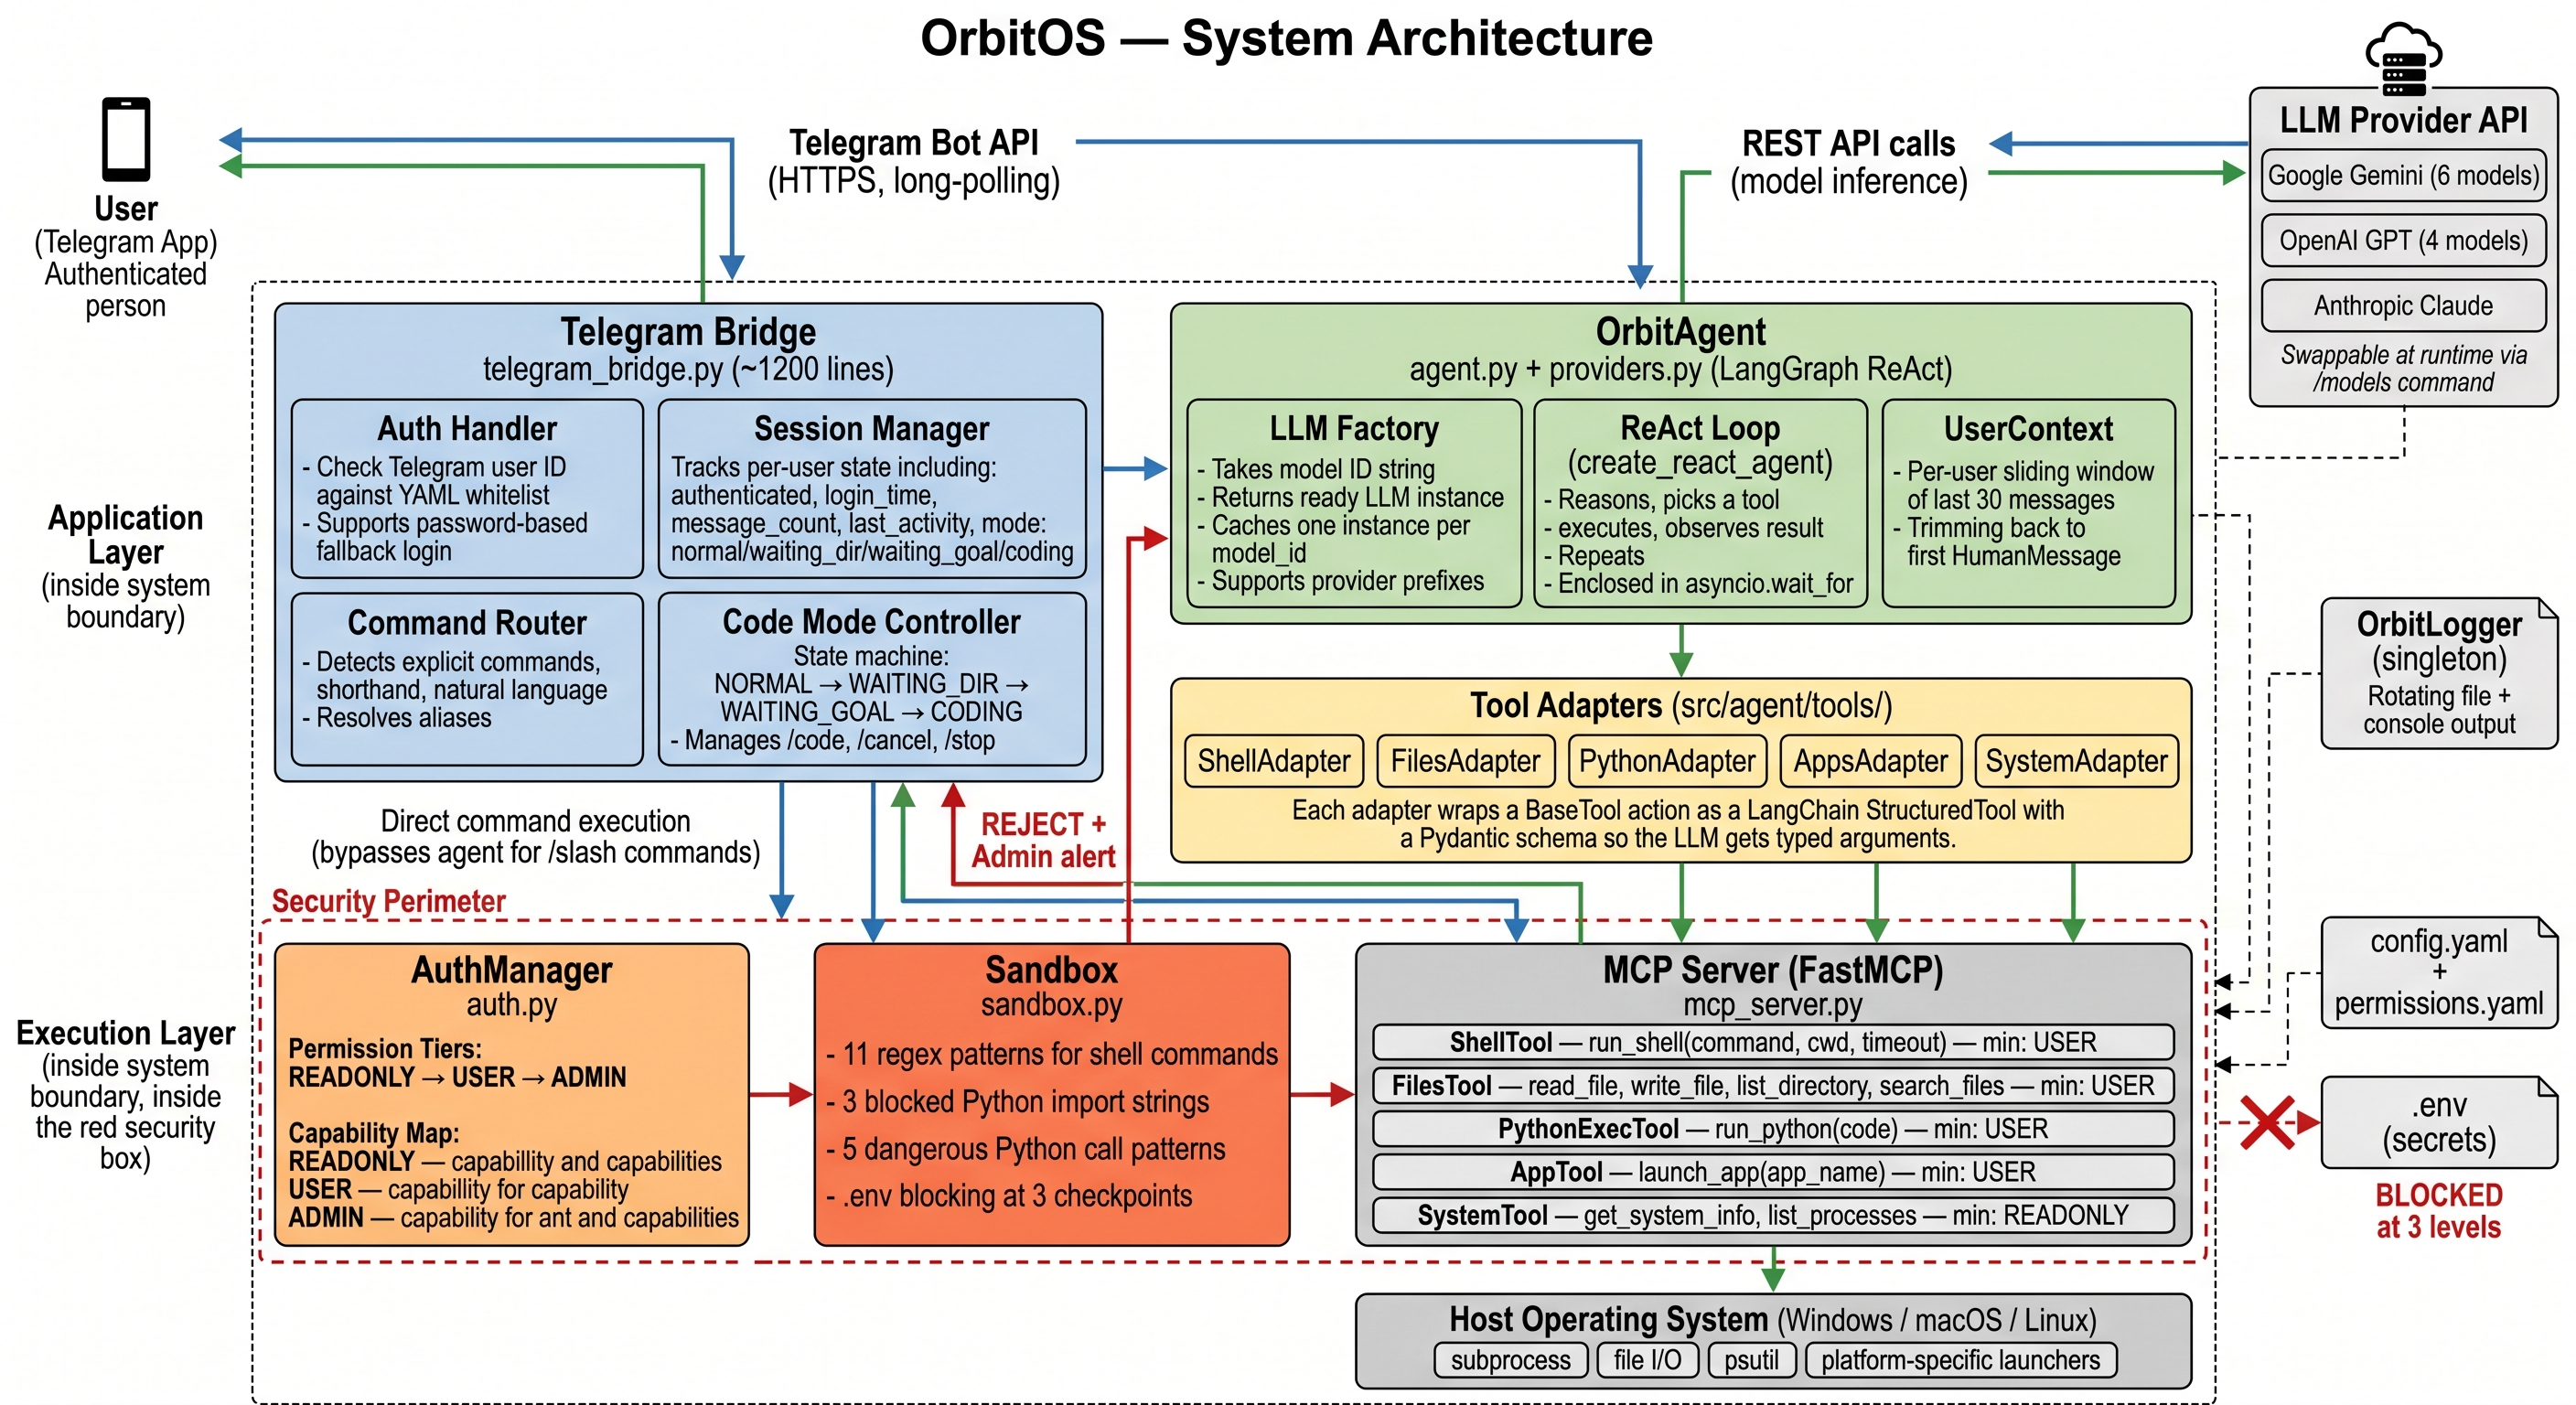
\includegraphics[width=0.92\textwidth]{system_architecture.png}
    \caption{High-Level System Architecture Diagram}
    \label{fig:system-architecture}
\end{figure}

\subsection*{Component Breakdown}
\begin{itemize}
    \item \textbf{Web Application}:
    \begin{itemize}
        \item ReactJS dashboard with role-based access control
        \item Biometric enrollment interface
        \item Security policy configuration
    \end{itemize}
    
    \item \textbf{Chrome Extension}:
    \begin{itemize}
        \item Content script injection for form detection
        \item Secure IPC channel for credential transfer
        \item Browser action panel with quick-access features
    \end{itemize}
\end{itemize}

\subsection*{Security Foundation}
\begin{itemize}
    \item \textbf{Encryption}: AES-256 for data-at-rest, TLS 1.3 for data-in-transit
    \item \textbf{Authentication}: WebAuthn-compliant biometric verification
    \item \textbf{Storage}: Multi-region replication with automatic failover
\end{itemize}

\chapter{Overall Description}
\label{chap:overall-description}

\section{Product Perspective}
\label{sec:product-perspective}
BioVault employs a microservices architecture designed for high availability and security compliance, comprising four core components:

\begin{itemize}
    \item \textbf{Frontend Layer}:
    \begin{itemize}
        \item ReactJS 18 with TypeScript for type-safe development
        \item State management using Redux Toolkit
        \item Chrome Extension built with Manifest V3 and Service Workers
        \item Responsive UI via Tailwind CSS with mobile-first approach
    \end{itemize}
    
    \item \textbf{Backend Services}:
    \begin{itemize}
        \item FastAPI 0.95+ with Python 3.10+
        \item ASGI server (Uvicorn) for async capabilities
        \item Redis-based rate limiting (100 req/min per user)
        \item JWT authentication with refresh token rotation
    \end{itemize}
    
    \item \textbf{Data Layer}:
    \begin{itemize}
        \item MongoDB 6.0+ with encrypted storage engine
        \item Time Series Collections for audit logging
        \item Change Streams for real-time synchronization
        \item Sharded cluster for horizontal scaling
    \end{itemize}
    
    \item \textbf{Cloud Infrastructure}:
    \begin{itemize}
        \item AWS S3 with SSE-KMS for biometric data
        \item Cloudinary Media Library for encrypted asset storage
        \item Vaultwarden for secret management
    \end{itemize}
\end{itemize}


\section{Product Functions}
\label{sec:product-functions}

\subsection{Core Functionalities}
\begin{itemize}
    \item \textbf{Multi-Factor Authentication}:
    \begin{itemize}
        \item WebAuthn-compliant biometric verification
        \item FIDO2 security key support
        \item Fallback TOTP (Time-based One-Time Password)
    \end{itemize}
    
    \item \textbf{Credential Management}:
    \begin{itemize}
        \item AES-256-GCM encryption with HKDF key derivation
        \item Secure password sharing with expiration policies
        \item Breach monitoring via HaveIBeenPwned API
    \end{itemize}
\end{itemize}

\subsection{Advanced Features}
\begin{itemize}
    \item \textbf{Browser Integration}:
    \begin{itemize}
        \item Content script injection for form detection
        \item Secure message passing using Window.postMessage()
        \item Declarative Net Request rules for form matching
    \end{itemize}
    
    \item \textbf{Enterprise Support}:
    \begin{itemize}
        \item SCIM 2.0 user provisioning
        \item SAML 2.0 single sign-on integration
        \item RBAC (Role-Based Access Control) with custom policies
    \end{itemize}
\end{itemize}

\section{User Characteristics}
\label{sec:user-characteristics}

\subsection{End User Profiles}
\begin{itemize}
    \item \textbf{General Users}:
    \begin{itemize}
        \item Password hygiene awareness score $>$ 70th percentile
        \item Average 25+ online accounts
        \item Primary use case: Personal credential management
    \end{itemize}
    
    \item \textbf{Enterprise Administrators}:
    \begin{itemize}
        \item Manage 500+ user accounts
        \item Require SOC 2 compliance reporting
        \item Audit trail retention (7 years minimum)
    \end{itemize}
    
    \item \textbf{Developers}:
    \begin{itemize}
        \item Integration via REST API and Webhooks
        \item SDK availability for custom implementations
        \item Rate limit: 1000 requests/minute (OAuth2 clients)
    \end{itemize}
\end{itemize}

\subsection{Administrative Roles}
\begin{itemize}
    \item \textbf{Security Officers}:
    \begin{itemize}
        \item Configure password policies (length, complexity)
        \item Manage HSM (Hardware Security Module) integrations
        \item Review SIEM (Security Information and Event Management) alerts
    \end{itemize}
    
    \item \textbf{Support Engineers}:
    \begin{itemize}
        \item Monitor system health via Grafana dashboards
        \item Respond to incidents within SLA (99.9% uptime)
        \item Manage certificate rotations (90-day cycle)
    \end{itemize}
\end{itemize}

\section{Operating Environment}
\label{sec:operating-environment}

\subsection{Client Requirements}
\begin{itemize}
    \item \textbf{Browsers}:
    \begin{itemize}
        \item Chrome 112+ (Chromium 112.0.5615.0)
        \item Firefox 102+ with WebExtensions support
        \item Safari 16.4+ on macOS 13+
    \end{itemize}
    
    \item \textbf{Hardware}:
    \begin{itemize}
        \item Webcam: 720p resolution minimum with auto-focus
        \item Microphone: 16-bit/44.1kHz sampling
        \item TPM 2.0 for secure enclave operations
    \end{itemize}
\end{itemize}

\subsection{Server Specifications}
\begin{itemize}
    \item \textbf{Production Environment}:
    \begin{itemize}
        \item AWS EC2 c6g.4xlarge instances (ARM64)
        \item Kubernetes 1.27+ cluster with auto-scaling
        \item Istio service mesh for traffic management
    \end{itemize}
    
    \item \textbf{Monitoring}:
    \begin{itemize}
        \item Prometheus 2.45+ metrics collection
        \item Loki 2.8+ for log aggregation
        \item AlertManager for PagerDuty integration
    \end{itemize}
\end{itemize}

\section{Design and Implementation Constraints}
\label{sec:design-constraints}

\subsection{Technical Constraints}
\begin{itemize}
    \item \textbf{Performance}:
    \begin{itemize}
        \item API latency $<$ 300ms (p99)
        \item Cold start time $<$ 1.5s (Chrome Extension)
        \item Vault decryption $<$ 800ms (10,000 credentials)
    \end{itemize}
    
    \item \textbf{Security}:
    \begin{itemize}
        \item FIPS 140-2 validated cryptographic modules
        \item Annual penetration testing requirements
        \item Secret rotation every 90 days
    \end{itemize}
\end{itemize}

\subsection{Compliance Requirements}
\begin{itemize}
    \item GDPR Article 32 (Data Protection by Design)
    \item NIST SP 800-63B Digital Identity Guidelines
    \item PCI DSS v4.0 for payment processing
\end{itemize}

\section{Assumptions and Dependencies}
\label{sec:assumptions}

\subsection{Key Assumptions}
\begin{itemize}
    \item Biometric sensor availability:
    \begin{itemize}
        \item 95\% of users have webcam/microphone
        \item 60\% of mobile devices have fingerprint sensors
    \end{itemize}
    
    \item Network conditions:
    \begin{itemize}
        \item Minimum 1 Mbps connection for biometric auth
        \item $<$5\% packet loss tolerance
    \end{itemize}
\end{itemize}

\subsection{Third-Party Dependencies}
\begin{itemize}
    \item \textbf{Critical Services}:
    \begin{itemize}
        \item AWS KMS for key management
        \item Cloudflare Workers for edge computing
        \item Twilio Verify for SMS 2FA
    \end{itemize}
    
    \item \textbf{Fallback Strategies}:
    \begin{itemize}
        \item 48-hour local credential cache
        \item Multi-cloud storage replication
        \\item Circuit breaker pattern implementation
    \end{itemize}
\end{itemize}

\chapter{Functional Requirements}
\section{User Registration and Authentication}
\subsection{User Registration}
\begin{itemize}
    \item \textbf{FR1}: Users register using a valid email and create a master password (for initial vault setup).
    \item \textbf{FR2}: The system must verify the uniqueness of the user’s email.
    \item \textbf{FR3}: Passwords are hashed using bcrypt before storage.
    \item \textbf{FR4}: Successful registration initializes an empty encrypted vault.
\end{itemize}

\subsection{User Login}
\begin{itemize}
    \item \textbf{FR5}: Users log in using their email and master password.
    \item \textbf{FR6}: After the initial authentication, a secondary biometric verification (face, voice, or fingerprint) is required.
    \item \textbf{FR7}: On successful login, a JWT token is issued to manage the user session.
    \item \textbf{FR8}: The system must handle invalid login attempts and provide appropriate error messages.
\end{itemize}

\section{Biometric Enrollment and Verification}
\begin{itemize}
    \item \textbf{FR9}: Users must enroll their biometric data (face, voice, fingerprint) through a guided interface.
    \item \textbf{FR10}: Biometric data is processed via deep learning algorithms and stored in encrypted form.
    \item \textbf{FR11}: Biometric verification is required during sensitive operations such as autofill or vault access.
\end{itemize}

\section{Password Management}
\subsection{Vault Operations}
\begin{itemize}
    \item \textbf{FR12}: Authenticated users can perform CRUD operations on their credentials.
    \item \textbf{FR13}: Passwords are encrypted locally (AES-256) before being synchronized with the backend.
    \item \textbf{FR14}: The system supports importing credentials through CSV file upload with proper schema validation.
\end{itemize}


\subsection{Use Case Diagram}
\begin{figure}[h]
    \centering
    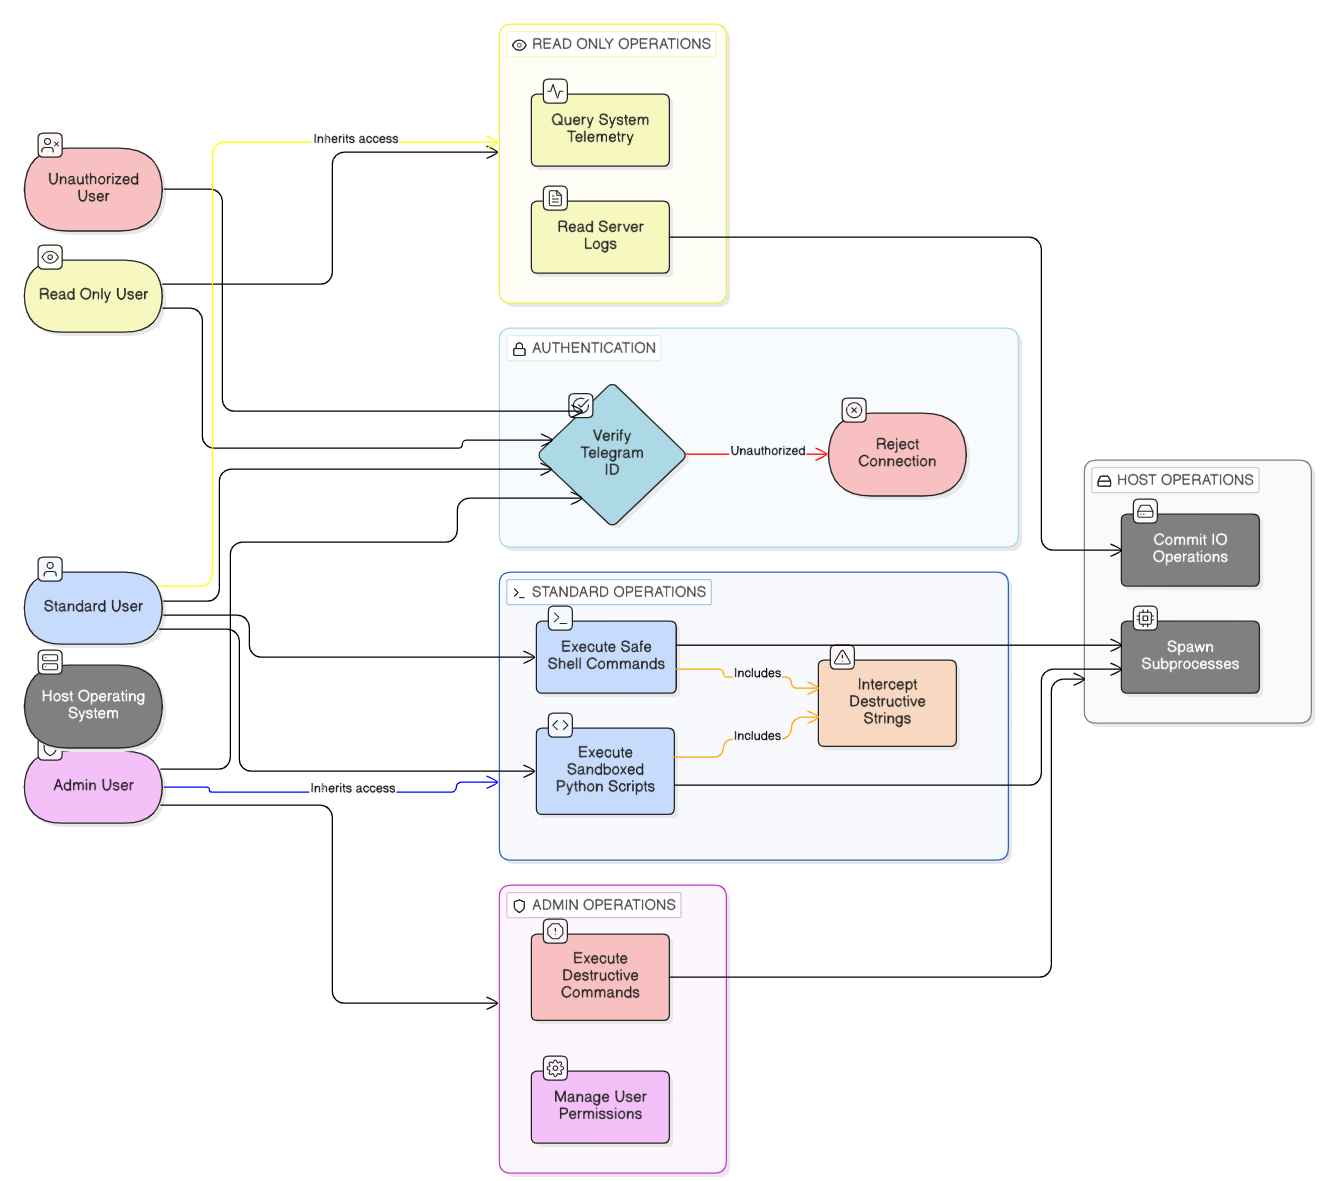
\includegraphics[width=\textwidth]{use_case_diagram.png}
    \caption{Use Case Diagram}
    \label{fig:use_case_diagram}
\end{figure}



\subsection{Autofill and Form-Filling}
\begin{itemize}
    \item \textbf{FR15}: The Chrome Extension detects login forms and prompts for biometric verification.
    \item \textbf{FR16}: On successful biometric confirmation, saved credentials are securely autofilled into detected fields.
\end{itemize}

\section{Subscription and Premium Features}
\begin{itemize}
    \item \textbf{FR17}: Users can upgrade to premium tiers to access advanced features such as detailed audit logs and enhanced biometric recovery.
    \item \textbf{FR18}: Payment processing and subscription status are managed using secure, token-based API calls.
\end{itemize}

\chapter{Non-Functional Requirements}
\section{Security}
\begin{itemize}
    \item \textbf{NFR1}: All data transmissions must occur over HTTPS.
    \item \textbf{NFR2}: Sensitive data (passwords and biometrics) must be encrypted using AES-256.
    \item \textbf{NFR3}: Implement rate limiting and input validation to prevent security threats (e.g., brute force, SQL injection, XSS).
    \item \textbf{NFR4}: JWT tokens must be securely generated and validated.
\end{itemize}

\section{Performance}
\begin{itemize}
    \item \textbf{NFR5}: API responses, including biometric verification, should complete within 500ms under normal load.
    \item \textbf{NFR6}: The user interface should remain responsive even during background data synchronization.
\end{itemize}

\section{Usability}
\begin{itemize}
    \item \textbf{NFR7}: The interface must be intuitive and accessible on both desktop and mobile devices.
    \item \textbf{NFR8}: Clear, responsive feedback should be provided during authentication and vault operations.
\end{itemize}

\section{Scalability and Maintainability}
\begin{itemize}
    \item \textbf{NFR9}: The system must support horizontal and vertical scaling to accommodate an increasing user base.
    \item \textbf{NFR10}: Code should follow modular design practices and be well-documented to simplify future maintenance.
\end{itemize}

\chapter{System Architecture and Interface Requirements}
\section{System Architecture}
BioVault follows a Model-View-Controller (MVC) architecture:
\begin{itemize}
    \item \textbf{Model}: MongoDB stores all user, credential, and biometric data in encrypted format.
    \item \textbf{View}: The ReactJS frontend provides a rich, responsive user interface.
    \item \textbf{Controller}: FastAPI handles the core business logic and API routing.
\end{itemize}

\subsection{Data Flow Diagram}
\begin{figure}[h]
    \centering
    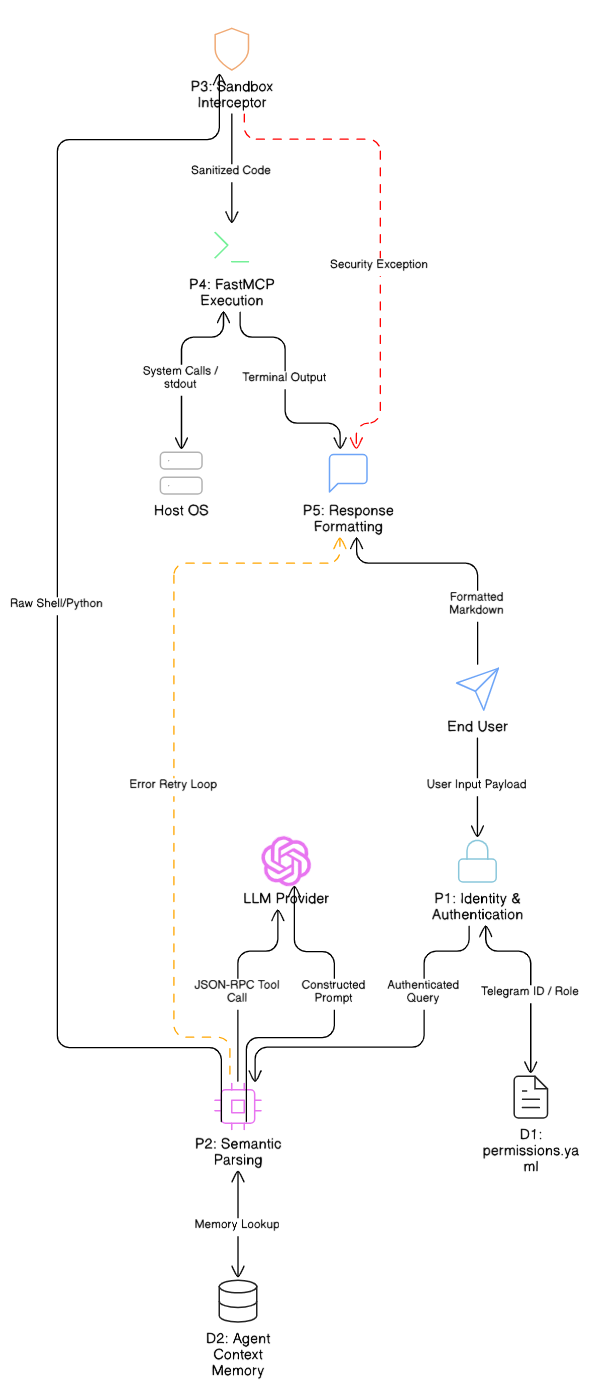
\includegraphics[width=\textwidth]{data_flow_diagram.jpg}
    \caption{Data Flow Diagram}
    \label{fig:data_flow_diagram}
\end{figure}

\section{External Interfaces}
\subsection{User Interfaces}
\begin{itemize}
    \item Responsive web pages for dashboard, vault management, biometric enrollment, and subscription details.
    \item A dedicated Chrome Extension UI to facilitate autofill and on-the-go authentication.
\end{itemize}

\subsection{Software Interfaces}
\begin{itemize}
    \item RESTful APIs support communication between the ReactJS frontend and FastAPI backend.
    \item Integration with third-party APIs for biometric authentication (e.g., WebAuthn) and cloud storage (Cloudinary).
\end{itemize}

\subsection{Communication Interfaces}
\begin{itemize}
    \item HTTP/HTTPS for secure web communication.
    \item JSON format for data exchange between client and server.
\end{itemize}

\chapter{Design Constraints}
\begin{itemize}
    \item \textbf{Technology Stack}: Must adhere to the use of ReactJS, FastAPI, MongoDB, and modern cloud services.
    \item \textbf{Security Practices}: Follow strict encryption and authentication measures as per industry standards.
    \item \textbf{Cross-Platform Compatibility}: Ensure seamless support for both web and Chrome Extension interfaces.
\end{itemize}

\chapter{Validation and Verification Requirements}
\section{Testing Strategy}
\begin{itemize}
    \item \textbf{Unit Testing}: Each module will be unit tested to verify individual functionalities.
    \item \textbf{Integration Testing}: Test interactions between modules such as authentication, biometric verification, and data synchronization.
    \item \textbf{System Testing}: Conduct end-to-end testing on both the web application and Chrome Extension.
    \item \textbf{User Acceptance Testing (UAT)}: Involve end-users in validating the overall usability and functionality.
\end{itemize}

\section{Acceptance Criteria}
\begin{itemize}
    \item All functional requirements are implemented and verified.
    \item The system meets performance benchmarks (API response times, UI responsiveness).
    \item Security audits confirm there are no critical vulnerabilities.
    \item User feedback from UAT is positive and suggests a user-friendly interface.
\end{itemize}

\chapter{Appendices}
\section{Glossary}
\begin{itemize}
    \item \textbf{JWT}: JSON Web Token.
    \item \textbf{AES-256}: Advanced Encryption Standard with 256-bit key.
    \item \textbf{CRUD}: Create, Read, Update, Delete.
    \item \textbf{MVC}: Model-View-Controller architectural pattern.
\end{itemize}

\section{System Diagrams}
\label{sec:system_diagrams}



\subsection{Entity-Relationship Diagram}
\begin{figure}[h]
    \centering
    \includegraphics[height=\textheight]{er_diagram.png}
    \caption{Entity-Relationship Diagram}
    \label{fig:er_diagram}
\end{figure}



\subsection{Sequence Diagram}
\begin{figure}[h]
    \centering
    \includegraphics[width=\textwidth]{sequence_diagram.png}
    \caption{Sequence Diagram}
    \label{fig:sequence_diagram}
\end{figure}

The system architecture and workflows are visualized through the following diagrams, which provide both high-level overviews and detailed operational perspectives:

\begin{itemize}


    \item \textbf{Figure \ref{fig:data_flow_diagram}}: Data Flow Diagram \\
    Details the movement of sensitive information through the system, emphasizing encryption/decryption points and secure channels between browser extension, web app, and cloud infrastructure.

    \item \textbf{Figure \ref{fig:er_diagram}}: Entity-Relationship Diagram \\
    Models the database structure showing relationships between core entities: Users, Vaults, Credentials, Biometric\_Templates, and Session\_Tokens. Includes cardinality constraints and primary/foreign keys.

    \item \textbf{Figure \ref{fig:use_case_diagram}}: Use Case Diagram \\
    Captures user-system interactions covering authentication flows, password management, biometric enrollment, and auto-fill operations. Identifies primary actors (Users, Admins) and system boundaries.

    \item \textbf{Figure \ref{fig:sequence_diagram}}: Sequence Diagram \\
    Demonstrates temporal aspects of critical operations including biometric authentication sequence, credential auto-fill process, and cross-device synchronization workflow.
    
\end{itemize}
\end{document}

% \begin{titlepage}
%     \begin{flushright}
%         \rule{16cm}{5pt}\vskip1cm
%         \begin{bfseries}
%             \Huge{SOFTWARE REQUIREMENTS\\ SPECIFICATION}\\
%             \vspace{1.5cm}
%             for\\
%             \vspace{1.5cm}
%             \Large{BioVault - Biometric Password Manager}\\
%             % \vspace{1.5cm}
%             % \LARGE{}\\
%             \vspace{1.5cm}
%             \Large{Prepared by :}\\
%             \vspace{0.5cm}
%             1. Tejaswini Durge (331020)\\
%             2. Arya Kadam (331028)\\
%             3. Chinmay Kale (331032)\\
%             4. Prasad Kute (331034)\\
%             \vspace{1.5cm}
%             \Large{Submitted to :}\\
%             \vspace{0.5cm}
%             Prof. (Mrs.) Priya Makarand Shelke \\
%             \vspace{1.5cm}
%             \Large{\today}\\
%         \end{bfseries}
%     \end{flushright}
% \end{titlepage}

% \tableofcontents
% \newpage

% \chapter{Introduction}
% \section{Purpose}
% The purpose of this Software Requirements Specification (SRS) document is to provide a detailed description of the requirements for the AI Based SWOC Analysis system. This system is intended to assist university students in obtaining insights into their overall Placement Readiness and identifying areas for skill improvement. Additionally, the system offers an administrative panel for authorized personnel to oversee and manage student profiles. This document outlines the functional and non-functional requirements, system features, and design constraints to ensure the successful development and deployment of the system.

% \section{Scope}
% The AI Based SWOC Analysis system is designed to help students manage and analyze their academic and extracurricular data to assess their strengths, weaknesses, opportunities, and challenges (SWOC) related to placements. Key functionalities include:
% \begin{itemize}
%     \item User registration and authentication.
%     \item Profile management for academic details, projects, internships, and coding platform statistics.
%     \item SWOC grade calculation based on predefined criteria.
%     % \item Integration with third-party coding platforms (LeetCode, GeeksforGeeks, Codeforces, Codechef, HackerRank) to fetch and synchronize coding statistics.
%     % \item Automated nightly data refresh and manual refresh options.
%     \item Administrative panel for managing student profiles.
%     \item Secure handling and storage of sensitive information.
%     \item Provide the Students with a Roadmap to  further enhance their skills.
% \end{itemize}

% \section{Definitions, Acronyms, and Abbreviations}
% \begin{itemize}
%     \item \textbf{SRS}: Software Requirements Specification
%     \item \textbf{SWOC}: Strengths, Weaknesses, Opportunities, Challenges (a calculated grade)
%     \item \textbf{API}: Application Programming Interface
%     % \item \textbf{AWS}: Amazon Web Services
%     \item \textbf{SGPA}: Semester Grade Point Average
%     \item \textbf{CGPA}: Cumulative Grade Point Average
%     \item \textbf{UI}: User Interface
%     \item \textbf{UX}: User Experience
%     \item \textbf{JWT}: JSON Web Token
%     \item \textbf{CRUD}: Create, Read, Update, Delete
%     \item \textbf{REST}: Representational State Transfer
% \end{itemize}

% \section{References}
% \begin{itemize}
%     % \item LeetCode API documentation: \url{https://leetcode.com/graphql}
%     % \item GFG API documentation: \url{https://gfg-api-fefa.onrender.com/USER_NAME}
%     % \item Codeforces API documentation: \url{https://codeforces.com/api/user.info?handles=USERNAME}
%     \item Project Repository: \url{https://github.com/kuteprasad/swoc_react_v4}
%     \item MongoDB Documentation: \url{https://docs.mongodb.com/}
%     \item Node.js Documentation: \url{https://nodejs.org/en/docs/}
%     \item Express.js Documentation: \url{https://expressjs.com/en/4x/api.html}
% \end{itemize}

% \section{System Overview}
% The AI Based SWOC Analysis system is a web-based application designed to provide students with a centralized platform to manage their academic records, project details and internships. Offering a comprehensive overview of a student's performance and achievements. The administrative panel ensures that authorized personnel can efficiently manage and oversee student profiles, maintaining data integrity and accuracy.

% \chapter{Overall Description}
% \section{Product Perspective}
% The AI Based SWOC Analysis system is an independent web application developed to serve as a centralized hub for student profile management. The system comprises a frontend developed using React, and a backend built with Node.js and Express.js, interfacing with a MongoDB database.

% \section{Product Functions}
% \begin{itemize}
%     \item \textbf{User Registration \& Authentication}: Users can create accounts using their Register ID and secure passwords, and authenticate themselves to access their profiles.
%     \item \textbf{Profile Management}: Students can input and update personal information, academic details, projects and internships.
%     \item \textbf{SWOC Grade Calculation}: The system calculates a SWOC grade based on predefined criteria involving academic performance and Projects.
%     % \item \textbf{Coding Platform Synchronization}: Integrates with APIs from LeetCode, GeeksforGeeks (GFG), Codeforces, Codechef, and HackerRank to fetch and update coding statistics.
%     % \item \textbf{Data Refresh Mechanism}: Provides nightly automated data synchronization with an option for manual refresh by the user.
%     \item \textbf{Administrative Panel}: Allows admins to manage and oversee student profiles, ensuring data accuracy and handling administrative tasks efficiently.
% \end{itemize}

% \section{User Characteristics}
% \subsection{Students}
% \begin{itemize}
%     \item Age Range: 18-25
%     \item Technical Proficiency: Basic to intermediate knowledge of web applications.
%     \item Goals: Manage academic records, track project and internship experiences and assess placement readiness.
% \end{itemize}

% \subsection{Administrators}
% \begin{itemize}
%     \item Age Range: 25-60
%     \item Technical Proficiency: Intermediate to advanced understanding of web systems.
%     \item Goals: Oversee student profiles, manage data integrity, and ensure the smooth operation of the System.
% \end{itemize}

% \section{Operating Environment}
% \begin{itemize}
%     \item \textbf{Frontend}: Compatible with major browsers (Chrome, Firefox, Safari, Edge) on desktop and mobile devices.
%     \item \textbf{Backend}: Node.js environment with Express.js framework.
%     \item \textbf{Database}: MongoDB.
%     % \item \textbf{Hosting}: Deployed on AWS EC2 instances or AWS Elastic Beanstalk for scalability.
%     % \item \textbf{Third-Party Services}: LeetCode, GFG, Codeforces, Codechef, and HackerRank APIs.
% \end{itemize}

% \section{Design and Implementation Constraints}
% \begin{itemize}
%     \item \textbf{Technology Stack}: Must use Node.js, Express.js, MongoDB, React and JavaScript for development.
%     % \item \textbf{API Availability}: Dependence on the availability and stability of third-party APIs for coding platform data.
%     % \item \textbf{Hosting Environment}: Must be deployed on AWS with considerations for cost and scalability.
%     \item \textbf{Security Standards}: Adherence to industry-standard security practices for data protection.
% \end{itemize}

% \section{Assumptions and Dependencies}
% \begin{itemize}
%     % \item Users have active accounts on the coding platforms they wish to synchronize.
%     % \item Third-party APIs remain stable and accessible throughout the system's lifecycle.
%     \item Internet connectivity is available for accessing the web application and third-party APIs.
%     \item Security measures like HTTPS are implemented to protect data during transmission.
% \end{itemize}

% \chapter{Functional Requirements}
% \section{User Registration and Authentication}
% \subsection{User Registration}
% \begin{itemize}
%     \item \textbf{FR1}: Users must be able to register using a unique Register ID, name, password, enrollment year, current year, and branch.
%     \item \textbf{FR2}: The system must validate the uniqueness of the Register ID during registration.
%     \item \textbf{FR3}: Passwords must be stored securely using encryption (e.g., bcrypt hashing).
%     \item \textbf{FR4}: Upon successful registration, users should receive a confirmation message and be redirected to the login page.
%     \item \textbf{FR5}: Input fields must be validated to ensure data integrity (e.g., valid email format, password strength).
% \end{itemize}

% \subsection{User Login}
% \begin{itemize}
%     \item \textbf{FR6}: Registered users must be able to log in using their Register ID and password.
%     \item \textbf{FR7}: The system must authenticate users by verifying the hashed password stored in the database.
%     \item \textbf{FR8}: Upon successful login, users should receive a JWT token for session management.
%     \item \textbf{FR9}: The system must handle failed login attempts gracefully, providing appropriate error messages.
%     % \item \textbf{FR10}: Implement rate limiting to prevent brute-force attacks on the login endpoint.
% \end{itemize}

% \section{Profile Management}
% \subsection{View Profile}
% \begin{itemize}
%     \item \textbf{FR10}: Authenticated users must be able to view their complete profile, including personal information, academic details, projects and  internships.
%     \item \textbf{FR11}: Profile information should be displayed in a user-friendly and organized manner.
% \end{itemize}

% \subsection{Edit Profile}
% \begin{itemize}
%     \item \textbf{FR12}: Users must be able to update their email, phone number, projects, internships, SGPA, and CGPA.
%     \item \textbf{FR13}: Core profile fields such as Register ID, Name, Enrollment Year, Branch, and SWOC Grade must be non-editable by the user.
%     \item \textbf{FR14}: The system must validate input data to ensure correctness (e.g., SGPA and CGPA within valid ranges).
%     \item \textbf{FR15}: Users should receive confirmation upon successful profile updates.
% \end{itemize}

% \section{SWOC Grade Calculation}
% \subsection{Automatic Calculation}
% \begin{itemize}
%     \item \textbf{FR16}: The system must automatically calculate the SWOC grade based on predefined criteria involving CGPA, SGPA, projects, and internships.
%     \item \textbf{FR17}: SWOC Grade must be displayed on the user profile and updated upon any relevant data changes.
% \end{itemize}

% % \section{Coding Platform Synchronization}
% % \subsection{Add Coding Profiles}
% % \begin{itemize}
% %     \item \textbf{FR19}: Users must be able to input and save their coding platform profile URLs (HackerRank, LeetCode, GFG, Codechef, Codeforces).
% %     \item \textbf{FR20}: The system should provide validation to ensure the correctness of the provided URLs.
% % \end{itemize}

% % \subsection{Fetch Coding Data}
% % \begin{itemize}
% %     \item \textbf{FR21}: The system must fetch data from the provided coding platform URLs using their respective APIs.
% %     \item \textbf{FR22}: Fetched data should include relevant statistics such as total problems solved, difficulty-wise problem counts, ratings, and rankings.
% %     \item \textbf{FR23}: The system must handle API rate limits and errors gracefully, ensuring data consistency.
% % \end{itemize}

% % \subsection{Store Coding Data}
% % \begin{itemize}
% %     \item \textbf{FR24}: Retrieved coding platform data must be stored in the user's profile within the MongoDB database.
% %     \item \textbf{FR25}: The system should ensure data integrity and prevent duplication or corruption during storage.
% % \end{itemize}

% % \section{Data Refresh Mechanism}
% % \subsection{Automated Refresh}
% % \begin{itemize}
% %     \item \textbf{FR26}: The system must automatically refresh coding platform data nightly to ensure up-to-date statistics.
% %     \item \textbf{FR27}: Implement scheduling mechanisms (e.g., cron jobs) to handle automated data synchronization.
% % \end{itemize}

% % \subsection{Manual Refresh}
% % \begin{itemize}
% %     \item \textbf{FR28}: Users must have the option to manually trigger a data refresh for their coding platform profiles.
% %     \item \textbf{FR29}: Upon initiating a manual refresh, the system must fetch and update the latest data from all linked coding platforms.
% %     \item \textbf{FR30}: Users should receive feedback on the success or failure of the manual refresh operation.
% % \end{itemize}

% \section{Administrative Panel}
% \subsection{Manage Student Profiles}
% \begin{itemize}
%     \item \textbf{FR18}: Admins must be able to view all student profiles.
%     \item \textbf{FR19}: Admins must have the ability to update or correct student profile data as needed.
%     \item \textbf{FR20}: Admins should be able to reset user passwords and manage user roles.
% \end{itemize}

% \subsection{User Role Management}
% \begin{itemize}
%     \item \textbf{FR21}: The system must support role-based access control, distinguishing between student and admin roles.
%     \item \textbf{FR22}: Only admins should have access to the administrative panel and its functionalities.
% \end{itemize}

% % \section{Coding Platform Data Synchronization}
% % \subsection{LeetCode}
% % \begin{itemize}
% %     \item \textbf{FR36}: Fetch and store total problems solved, and count by difficulty (Easy, Medium, Hard).
% %     \item \textbf{FR37}: Update LeetCode rank and other relevant statistics.
% % \end{itemize}

% % \subsection{GeeksforGeeks (GFG)}
% % \begin{itemize}
% %     \item \textbf{FR38}: Fetch and store institute rank, total problems solved, and difficulty-wise counts.
% % \end{itemize}

% % \subsection{Codeforces}
% % \begin{itemize}
% %     \item \textbf{FR39}: Fetch and store current rating, max rating, and total problems solved.
% % \end{itemize}

% % \subsection{Codechef}
% % \begin{itemize}
% %     \item \textbf{FR40}: Fetch and store current rating and total problems solved.
% % \end{itemize}

% % \subsection{HackerRank}
% % \begin{itemize}
% %     \item \textbf{FR41}: Fetch and store profile details as available.
% % \end{itemize}

% \chapter{Non-Functional Requirements}
% % \section{Performance Requirements}
% % \begin{itemize}
% %     \item \textbf{NFR1}: The system should support at least 500 concurrent users without performance degradation.
% %     \item \textbf{NFR2}: Profile data retrieval and updates should be processed within 2 seconds.
% %     \item \textbf{NFR3}: The system should handle API rate limits gracefully, ensuring data consistency.
% % \end{itemize}

% \section{Security}
% \begin{itemize}
%     \item \textbf{NFR1}: All sensitive data transmissions must use HTTPS to ensure data encryption during transit.
%     \item \textbf{NFR2}: Passwords must be stored securely using industry-standard encryption algorithms (e.g., bcrypt).
%     \item \textbf{NFR3}: Implement input validation and sanitation to prevent common security vulnerabilities like SQL injection and cross-site scripting (XSS).
%     \item \textbf{NFR4}: JWT tokens must be securely generated and validated to manage user sessions.
%     \item \textbf{NFR5}: Regular security audits and vulnerability assessments must be conducted.
% \end{itemize}

% % \section{Reliability}
% % \begin{itemize}
% %     \item \textbf{NFR9}: The system must achieve 99.9\% uptime, ensuring high availability for users.
% %     \item \textbf{NFR10}: Implement backup and recovery mechanisms to prevent data loss.
% %     \item \textbf{NFR11}: Ensure failover strategies are in place for critical components.
% % \end{itemize}

% \section{Usability}
% \begin{itemize}
%     \item \textbf{NFR6}: The user interface should be intuitive and user-friendly, requiring minimal training for new users.
%     \item \textbf{NFR7}: The system should be responsive, providing an optimal experience on both desktop and mobile devices.
%     % \item \textbf{NFR14}: Accessibility standards (e.g., WCAG) should be followed to ensure the system is usable by individuals with disabilities.
% \end{itemize}

% % \section{Scalability}
% % \begin{itemize}
% %     \item \textbf{NFR15}: The system architecture should support horizontal and vertical scaling to accommodate growth in user base and data volume.
% %     \item \textbf{NFR16}: Database indexing and optimization techniques should be employed to ensure efficient data retrieval and storage.
% %     \item \textbf{NFR17}: Utilize cloud services like AWS Auto Scaling and Load Balancing to manage increased loads.
% % \end{itemize}

% \section{Maintainability}
% \begin{itemize}
%     \item \textbf{NFR8}: The codebase should follow consistent coding standards and best practices to facilitate easy maintenance and updates.
%     \item \textbf{NFR9}: Comprehensive documentation should be provided for both the code and the system functionalities.
%     % \item \textbf{NFR20}: Modular architecture to allow independent updates and scaling of components.
% \end{itemize}

% \section{Compliance}
% \begin{itemize}
%     % \item \textbf{NFR21}: The system must comply with relevant data protection regulations (e.g., GDPR) to ensure user data privacy and security.
%     % \item \textbf{NFR22}: Adhere to industry standards for software development and deployment.
%     \item \textbf{NFR10}: Ensure compliance with university policies and guidelines regarding student data management.
% \end{itemize}

% \chapter{System Features}
% \section{User Registration \& Authentication}
% \subsection{Description}
% Students can create accounts by providing necessary personal and academic details. Secure authentication mechanisms ensure that only authorized users can access their profiles.

% \subsection{Functional Requirements}
% \begin{itemize}
%     \item \textbf{FR1}: User registration with unique Register ID.
%     \item \textbf{FR2}: Secure password storage using encryption.
%     \item \textbf{FR3}: User login with JWT-based session management.
%     \item \textbf{FR4}: Password reset functionality
% \end{itemize}

% \section{Profile Management}
% \subsection{Description}
% Users can manage their academic records, projects and internships.

% \subsection{Functional Requirements}
% \begin{itemize}
%     \item \textbf{FR5}: Add and update personal information.
%     \item \textbf{FR6}: Manage academic details including SGPA and CGPA.
%     \item \textbf{FR7}: Input and edit project and internship details.
%     % \item \textbf{FR8}: Link and synchronize coding platform profiles.
%     \item \textbf{FR8}: View aggregated data on a dashboard.
% \end{itemize}

% \section{SWOC Grade Calculation}
% \subsection{Description}
% The system calculates the SWOC grade based on predefined criteria involving academic performance.

% \subsection{Functional Requirements}
% \begin{itemize}
%     \item \textbf{FR9}: Automatic calculation of SWOC grade upon data updates.
%     \item \textbf{FR10}: Display SWOC grade on the user profile.
%     \item \textbf{FR11}: Provide suggestions for improvement based on SWOC analysis.
% \end{itemize}

% % \section{Coding Platform Synchronization}
% % \subsection{Description}
% % Integration with third-party coding platforms to fetch and display user statistics within the SPMS.

% % \subsection{Functional Requirements}
% % \begin{itemize}
% %     \item \textbf{FR13}: Input and store coding platform profile URLs.
% %     \item \textbf{FR14}: Fetch data from LeetCode, GFG, Codeforces, Codechef, and HackerRank.
% %     \item \textbf{FR15}: Store fetched data in MongoDB.
% %     \item \textbf{FR16}: Provide options for automatic and manual data refresh.
% %     \item \textbf{FR17}: Handle API rate limits and errors gracefully.
% % \end{itemize}

% % \section{Data Refresh Mechanism}
% % \subsection{Description}
% % Provides mechanisms for both automated and manual synchronization of coding platform data to ensure up-to-date statistics.

% % \subsection{Functional Requirements}
% % \begin{itemize}
% %     \item \textbf{FR18}: Schedule nightly automated data synchronization using cron jobs or similar scheduling tools.
% %     \item \textbf{FR19}: Allow users to manually trigger data synchronization through the user interface.
% %     \item \textbf{FR20}: Notify users upon successful or failed data synchronization attempts.
% % \end{itemize}

% \section{Administrative Panel}
% \subsection{Description}
% Admins can manage student profiles, ensuring data accuracy and handling administrative tasks efficiently.

% \subsection{Functional Requirements}
% \begin{itemize}
%     \item \textbf{FR12}: View all student profiles in a consolidated dashboard.
%     \item \textbf{FR13}: Edit and update student profile data as needed.
%     \item \textbf{FR14}: Reset user passwords and manage user roles.
%     \item \textbf{FR15}: Generate reports on student performance and SWOC grades.
% \end{itemize}

% \chapter{External Interface Requirements}
% \section{User Interfaces}
% \subsection{Student Interface}
% \begin{itemize}
%     \item Responsive web pages for profile viewing and management.
%     \item Forms for data input and updates.
%     \item Dashboard displaying aggregated academic data.
% \end{itemize}
% \begin{figure}[h]
%     \centering
%     \includegraphics[width=\textwidth]{dashboard.png}
%     \caption{Student Dashboard}
%     \label{fig:student_dashboard}
% \end{figure}

% \subsection{Admin Interface}
% \begin{itemize}
%     \item Secure login for admin users.
%     \item Overview of all student profiles.
%     \item Tools for editing and managing student data.
% \end{itemize}
% \begin{figure}[h]
%     \centering
%     \includegraphics[width=\textwidth]{admin_panel.png}
%     \caption{Admin Panel}
%     \label{fig:admin_panel}
% \end{figure}

% % \section{Hardware Interfaces}
% % \begin{itemize}
% %     \item Servers hosted on AWS EC2 instances.
% %     \item Interaction with external hardware if necessary (e.g., biometric authentication devices).
% % \end{itemize}

% \section{Software Interfaces}
% \begin{itemize}
%     \item Integration with MongoDB for database management.
%     % \item Interaction with third-party APIs for coding platform data synchronization.
%     \item RESTful APIs for frontend-backend communication.
% \end{itemize}

% \section{Communication Interfaces}
% \begin{itemize}
%     \item HTTP/HTTPS protocols for secure data transmission.
%     % \item WebSockets for real-time data updates if required.
%     \item JSON format for data exchange between client and server.
% \end{itemize}

% \chapter{System Architecture}
% \section{Overview}
% The AI Based SWOC Analysis system follows a Model-View-Controller (MVC) architecture to separate concerns and enhance maintainability. The system comprises the following components:
% \begin{itemize}
%     \item \textbf{Frontend}: Developed using React and JavaScript, providing an interactive user interface.
%     \item \textbf{Backend}: Built with Node.js and Express.js, handling system logic and database interactions.
%     \item \textbf{Database}: MongoDB stores user profiles, academic data, projects, internships.
%     % \item \textbf{Hosting}: AWS services ensure scalability, reliability, and secure deployment.
% \end{itemize}

% %\section{Component Diagram}
% %\begin{figure}[h]
% %    \centering
% %    \includegraphics[width=\textwidth]{component_diagram.png}
% %    \caption{System Component Diagram}
% %    \label{fig:component_diagram}
% %\end{figure}

% \section{Data Flow Diagram}
% \begin{figure}[h]
%     \centering
%     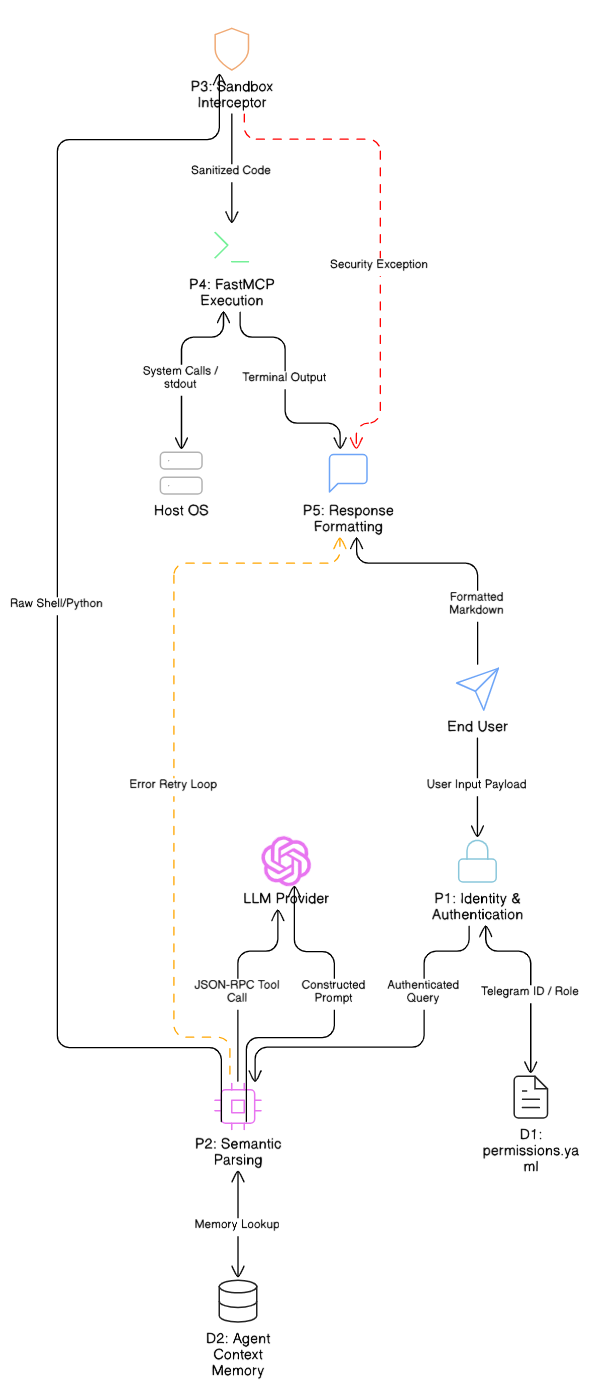
\includegraphics[width=250]{data_flow_diagram.png}
%     \caption{Data Flow Diagram}
%     \label{fig:data_flow_diagram}
% \end{figure}

% \section{Entity-Relationship Diagram}
% \begin{figure}[h]
%     \centering
%     \includegraphics[width=\textwidth]{er_diagram.png}
%     \caption{Entity-Relationship Diagram}
%     \label{fig:er_diagram}
% \end{figure}

% \section{Use Case Diagram}
% \begin{figure}[h]
%     \centering
%     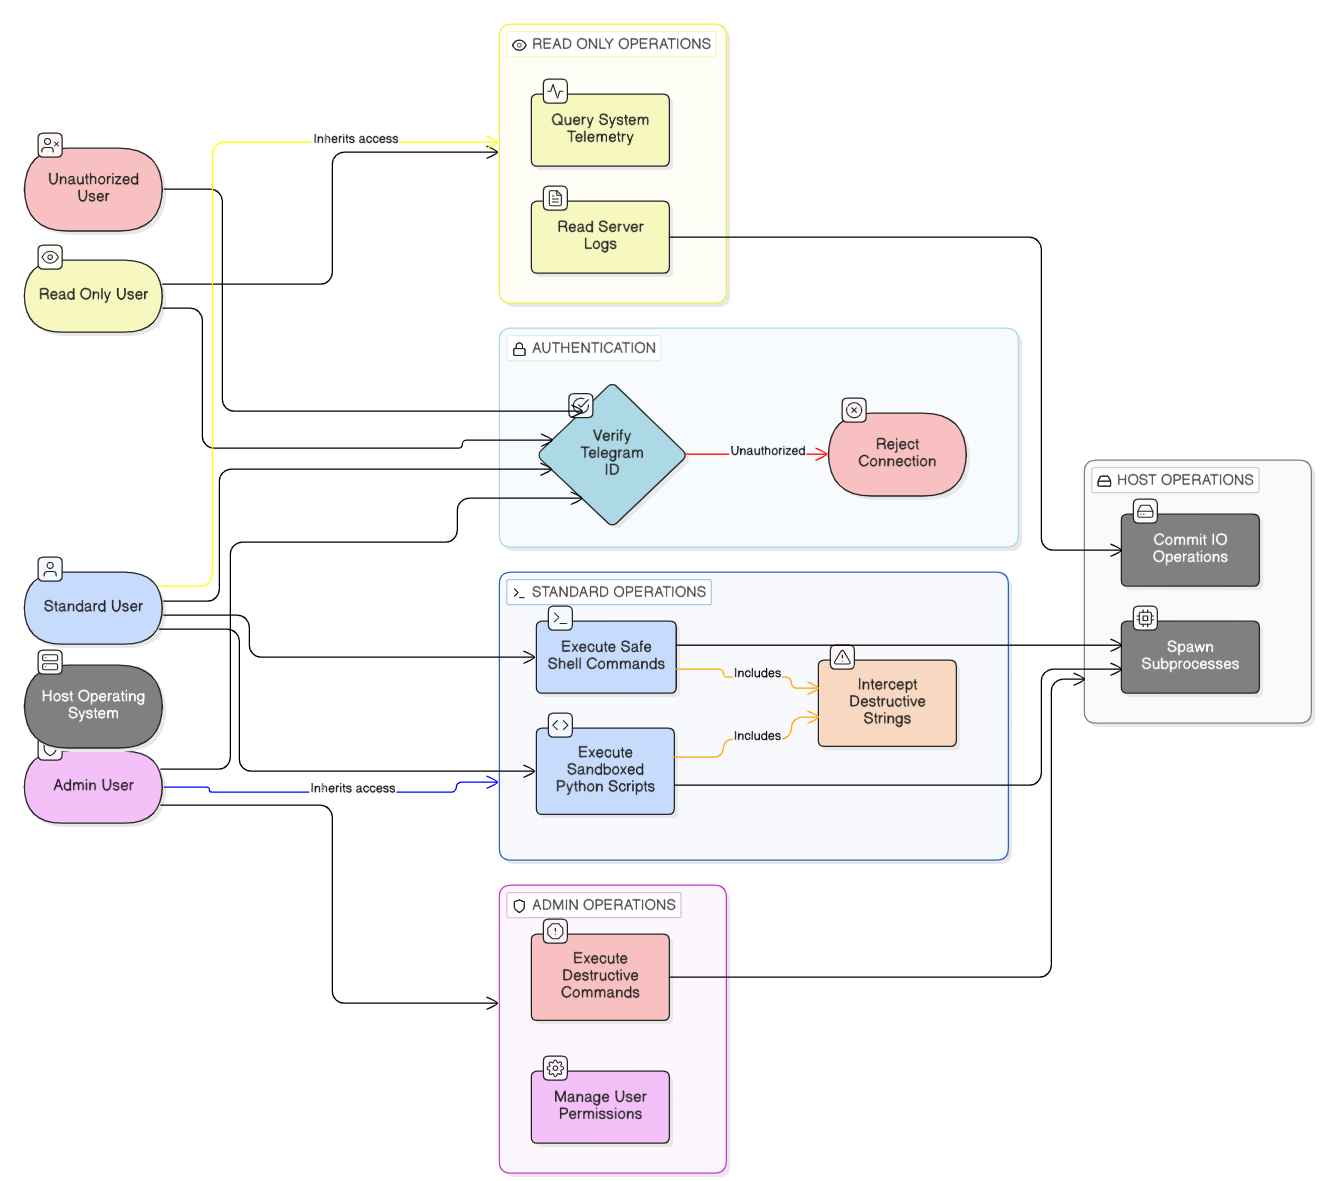
\includegraphics[width=\textwidth]{use_case_diagram.png}
%     \caption{Use Case Diagram}
%     \label{fig:use_case_diagram}
% \end{figure}

% \section{Sequence Diagram}
% \begin{figure}[h]
%     \centering
%     \includegraphics[width=\textwidth]{sequence_diagram.png}
%     \caption{Sequence Diagram}
%     \label{fig:sequence_diagram}
% \end{figure}

% % \section{Deployment Diagram}
% % \begin{figure}[h]
% %     \centering
% %     \includegraphics[width=\textwidth]{deployment_diagram.png}
% %     \caption{Deployment Diagram}
% %     \label{fig:deployment_diagram}
% % \end{figure}

% \chapter{Design Constraints}
% \begin{itemize}
%     \item \textbf{Technology Stack}: Must use Node.js, Express.js, MongoDB, React and JavaScript for development.
%     % \item \textbf{API Availability}: Dependence on the availability and stability of third-party APIs for coding platform data.
%     % \item \textbf{Hosting Environment}: Must be deployed on AWS with considerations for cost and scalability.
%     % \item \textbf{Security Standards}: Adherence to industry-standard security practices for data protection.
%     \item \textbf{Browser Compatibility}: Ensure compatibility across major browsers and devices.
%     \item \textbf{Performance Constraints}: Must handle data synchronization efficiently to prevent performance bottlenecks.
% \end{itemize}

% % \chapter{Validation \& Verification Requirements}
% % \section{Testing Requirements}
% % \begin{itemize}
% %     \item \textbf{Unit Testing}: Conduct unit tests for individual components and functions to ensure they work as intended.
% %     \item \textbf{Integration Testing}: Test interactions between different modules, such as frontend-backend communication and API integrations.
% %     \item \textbf{System Testing}: Validate that the entire system meets the specified requirements and works seamlessly.
% %     \item \textbf{User Acceptance Testing (UAT)}: Engage a group of end-users to test the system's functionality and usability, ensuring it meets their needs.
% %     \item \textbf{Performance Testing}: Assess the system's performance under various loads to ensure it meets performance requirements.
% %     \item \textbf{Security Testing}: Conduct vulnerability assessments and penetration testing to identify and mitigate security risks.
% % \end{itemize}

% % \section{Verification Procedures}
% % \begin{itemize}
% %     \item \textbf{Code Reviews}: Regular code reviews to ensure code quality and adherence to coding standards.
% %     \item \textbf{Automated Testing}: Implement automated testing frameworks (e.g., Jest for backend, Cypress for frontend) to streamline testing processes.
% %     \item \textbf{Manual Testing}: Perform manual testing for UI/UX aspects and complex scenarios that require human judgment.
% %     \item \textbf{Continuous Integration/Continuous Deployment (CI/CD)}: Utilize CI/CD pipelines to automate testing and deployment, ensuring rapid and reliable releases.
% % \end{itemize}

% % \section{Acceptance Criteria}
% % \begin{itemize}
% %     \item \textbf{Functional Completeness}: All functional requirements are implemented and working as specified.
% %     \item \textbf{Performance Benchmarks}: The system meets all defined performance requirements under expected loads.
% %     \item \textbf{Security Standards}: The system is free from critical security vulnerabilities and complies with data protection regulations.
% %     \item \textbf{User Satisfaction}: Users find the system intuitive, responsive, and valuable in managing their profiles and assessing placement readiness.
% %     \item \textbf{Reliability and Availability}: The system maintains high uptime and recovers gracefully from failures.
% % \end{itemize}

% % \chapter{Risk Analysis}
% % \section{Potential Risks}
% % \begin{itemize}
% %     \item \textbf{API Downtime}: Reliance on third-party APIs may lead to data fetch failures if APIs are unavailable.
% %     \item \textbf{Data Privacy}: Handling sensitive academic and personal data requires strict adherence to privacy regulations.
% %     \item \textbf{Scalability Issues}: Increased user load may affect system performance if not properly scaled.
% %     \item \textbf{Security Vulnerabilities}: Potential threats like SQL injection, XSS, and data breaches.
% %     \item \textbf{Data Inconsistency}: Synchronization issues between the system and third-party APIs could lead to inconsistent data.
% %     \item \textbf{Project Delays}: Development delays due to unforeseen technical challenges or resource constraints.
% % \end{itemize}

% % \section{Mitigation Plans}
% % \begin{itemize}
% %     \item \textbf{API Downtime}: Implement fallback mechanisms and data caching to handle API downtimes gracefully.
% %     \item \textbf{Data Privacy}: Ensure compliance with data privacy laws like GDPR through data encryption and secure storage practices.
% %     \item \textbf{Scalability Issues}: Design a scalable architecture using AWS services like Auto Scaling and Load Balancing to manage increased loads.
% %     \item \textbf{Security Vulnerabilities}: Conduct regular security audits, employ input validation, and use security best practices to mitigate vulnerabilities.
% %     \item \textbf{Data Inconsistency}: Implement robust error handling and data validation mechanisms to maintain data consistency.
% %     \item \textbf{Project Delays}: Establish realistic project timelines, allocate sufficient resources, and conduct regular progress reviews to prevent delays.
% % \end{itemize}

% \chapter{Appendices}
% \section{Glossary}
% \begin{itemize}
%     \item \textbf{JWT}: JSON Web Token
%     \item \textbf{CRUD}: Create, Read, Update, Delete
%     \item \textbf{REST}: Representational State Transfer
%     \item \textbf{UI}: User Interface
%     \item \textbf{UX}: User Experience
%     \item \textbf{API}: Application Programming Interface
%     \item \textbf{SWOC}: Strengths, Weaknesses, Opportunities, Challenges
%     \item \textbf{SRS}: Software Requirements Specification
% \end{itemize}

% \section{System Diagrams}
% \begin{itemize}
%     % \item \textbf{Figure \ref{fig:component_diagram}}: System Component Diagram
%     \item \textbf{Figure \ref{fig:data_flow_diagram}}: Data Flow Diagram
%     \item \textbf{Figure \ref{fig:er_diagram}}: Entity-Relationship Diagram
%     \item \textbf{Figure \ref{fig:use_case_diagram}}: Use Case Diagram
%     \item \textbf{Figure \ref{fig:sequence_diagram}}: Sequence Diagram
%     % \item \textbf{Figure \ref{fig:deployment_diagram}}: Deployment Diagram
% \end{itemize}

% % \section{Version Control}
% % \begin{tabular}{|c|c|c|c|}
% %     \hline
% %     \textbf{Version} & \textbf{Date} & \textbf{Author} & \textbf{Description} \\
% %     \hline
% %     1.0 & \today & Tejaswini Durge & Initial SRS Document \\
% %     \hline
% % \end{tabular}

% \end{document}